% ****** Start of file apssamp.tex ******
%
%   This file is part of the APS files in the REVTeX 4.2 distribution.
%   Version 4.2a of REVTeX, December 2014
%
%   Copyright (c) 2014 The American Physical Society.
%
%   See the REVTeX 4 README file for restrictions and more information.
%
% TeX'ing this file requires that you have AMS-LaTeX 2.0 installed
% as well as the rest of the prerequisites for REVTeX 4.2
%
% See the REVTeX 4 README file
% It also requires running BibTeX. The commands are as follows:
%
%  1)  latex apssamp.tex
%  2)  bibtex apssamp
%  3)  latex apssamp.tex
%  4)  latex apssamp.tex
%
\documentclass[%
 reprint,
%superscriptaddress,
%groupedaddress,
%unsortedaddress,
%runinaddress,
%frontmatterverbose, 
%preprint,
%preprintnumbers,
%nofootinbib,
%nobibnotes,
%bibnotes,
 amsmath,amssymb,
 aps,
 pra,
%prb,
%rmp,
%prstab,
%prstper,
%floatfix,
]{revtex4-2}
\usepackage[spanish,es-nodecimaldot]{babel}
\usepackage{color,soul}
\usepackage{physics}
\usepackage{minted}
\usepackage{graphicx}% Include figure files
%\usepackage{svg}
\usepackage{dcolumn}% Align table columns on decimal point
\usepackage{bm}% bold math
\usepackage{hyperref}% add hypertext capabilities
\definecolor{linkcolour}{rgb}{0,0.2,0.6} % Link color
\hypersetup{colorlinks,citecolor=linkcolour,breaklinks,urlcolor=linkcolour,linkcolor=linkcolour}
\usepackage{color,soul}
\usepackage{soulutf8}
\usepackage{mathrsfs}
\usepackage{wrapfig}
%\usepackage[mathlines]{lineno}% Enable numbering of text and display math
%\linenumbers\relax % Commence numbering lines

%\usepackage[showframe,%Uncomment any one of the following lines to test 
%%scale=0.7, marginratio={1:1, 2:3}, ignoreall,% default settings
%%text={7in,10in},centering,
%%margin=1.5in,
%%total={6.5in,8.75in}, top=1.2in, left=0.9in, includefoot,
%%height=10in,a5paper,hmargin={3cm,0.8in},
%]{geometry}

\begin{document}

\preprint{APS/123-QED}

\title{Modelo de Ising:\texorpdfstring{\\}{ }Apreciaciones Generales y Algoritmo Metrópolis.}% Force line breaks with \\

\author{Juan Esteban Aristizabal Zuluaga}
\affiliation{Instituto de Física, Universidad de Antioquia.}%Lines break automatically or can be forced with \\

\date{\today}% It is always \today, today,
             %  but any date may be explicitly specified

\begin{abstract}
Presentamos en este artículo un estudio medianamente detallado del modelo de Ising 2-dimensional en retícula cuadrada de lado $L$ con condiciones de frontera periódicas. Introducimos el sistema en general y hacemos un estudio por enumeración exacta de los microestados del sistema hasta un tamaño $L \times L = 5 \times 5$. Estudiamos el fenómeno de transición de fase de segundo orden para estos sistemas de $L$ pequeños y evidenciamos la complejidad computacional de la enumeración exacta para este modelo. Con esto en mente, se realiza un muestreo inteligente de los microestados del sistema con la implementación del algoritmo Metrópolis para el modelo en cuestión, el cual permite subir el valor de $L$ hasta $128$. En el algoritmo metrópolis notamos la importancia de la termalización del sistema y logramos evidenciar de primera mano el comienzo de la formación de la discontinuidad en el calor específico $c_v$, lo cual es característica de una transición de fase de segundo orden. 
\begin{description}
\item[Palabras clave] Modelo de Ising, conteo de microestados, ensamble canónico, calor específico,\\transición de fase, algoritmo metrópolis, termalización.
\end{description}
\end{abstract}

%\keywords{Suggested keywords}%Use showkeys class option if keyword
                              %display desired
\maketitle

%\tableofcontents
\onecolumngrid

\section{Consideraciones teóricas\label{sec:teoria-microestados}}


	\subsection{Hamiltoniano del sistema y ensamble canónico.\label{subsec:teoria-hamiltoniano}}
	
	El hamiltoniano del modelo de Ising está dado por
		\begin{equation}
			H = -J\sum_{\langle ij \rangle} \sigma_i \sigma_j, \label{eq:hamiltoniano}
		\end{equation}
	donde $\sigma_i = \pm 1$ (se conoce como espín),  $\langle ij \rangle$ da cuenta de interacción entre primeros vecinos y $J$ es la fuerza de la interacción entre primeros vecinos.

	El modelo de Ising asume que los espines están fijos en sus posiciones y puede ser aplicado en cualquier dimensionalidad y con cualquier tipo de rejilla. En nuestro caso nos centraremos en el sistema 2-dimensional con rejilla cuadrada de lado $L$. Es decir, estudiaremos la interacción del modelo de ising entre $N = L \times L$ espines. Las condiciones de frontera del sistema pueden ser de diversos tipos. En este trabajo usaremos más que todo las condiciones de frontera periódicas y mencionaremos algunas diferencias interesantes que emergen al considerar condiciones de frontera libres. Además, trabajaremos en unidades de $J=k_B=1$.

	Cuando el sistema está inmerso en un baño térmico, podemos trabajar en el ensamble canónico. La función partición está dada por 
		\begin{equation}
			Z(\beta) = \sum_n  e^{-\beta E_n}, 
		\end{equation}
	donde $E_n$ representa cada nivel de energía del sistema. Si el microestado $E_n = E$ tiene degeneración $\Omega(E)$ es claro que
		\begin{equation}
			Z(\beta) = \sum_E \Omega(E) e^{-\beta E}.
		\end{equation}
	Notemos que esta última expresión es conceptualmente muy útil, ya que vemos que las contribuciones a la función partición se pueden agrupar de acuerdo a las diferentes energías del sistema, via su degeneración $\Omega(E)$. En esta misma línea, sabemos también que probabilidad de que el sistema esté en un nivel de energía $E_n$, $p_n$, está dada por
		\begin{equation}
			p_n = \frac{e^{-\beta E_n}}{Z}
		\end{equation}
	y la probabilidad de que el sistema tenga energía $E$ está dada por
		\begin{equation}
			p_E = \frac{\Omega(E) e^{-\beta E}}{Z}. \label{eq:energy_prob}
		\end{equation}

	Cuando tenemos este sistema en el ensamble canónico y $L$ es lo suficientemente grande, se presenta una transición de fase de segundo orden caracterizada por una discontinuidad en el calor específico $c_v$ y se da a una temperatura crítica $T_c$. Cuando $L\rightarrow\infty$, se tiene $T_c = 2 / \log\left( 1 + \sqrt{2} \right) \approx 2.269$ \cite{Huang}.

	A pesar de que la escencia del modelo de Ising es muy sencilla, nos encontramos con un problema importante al estudiarlo (que se encuentra en gran parte de la física estadística), el cual es el conteo de microestados. El número de microestados del sistema 2-dimensional en rejilla cuadrada es $\Omega = 2^{L \times L}$. Para el caso $L=10$ esto es $\Omega \approx 10^{30} $. El cálculo del total de éste número de microestados rebasa cualquier capacidad computacional disponible hasta el momento.
	Entre otras cosas, para darnos una idea de este problema, estudiaremos en las siguientes secciones el cálculo de los microestados por enumeración exacta.

	\subsection{Microestados y contribuciones a la función partición\label{subsec:teoria-contribuciones-Z}}

	Los microestados explícitos, es decir, las $\Omega = 2^{L \times L}$ configuraciones posbiles en nuestro sistems son isomorfas a los primeros $\Omega$ números binarios. Con esta estrategia se pueden generar todas las configuraciones posibles, cambiando los dígitos que tengan valor $0$ de los números binarios por el valor $-1$. Una vez generadas todas las configuraciones para un $L$ dado, se puede calcular la energía de cada uno de ellos usando la expresión \ref{eq:hamiltoniano} y con ellas, se pueden calcular los $\Omega(E)$.

	\textit{Nota}: el código con el que se generaron las figuras se puede ver en el apéndice \ref{appx:microestados} y usa un módulo propio que escribimos, el cual contiene todas las funciones necesarias para generar las gráficas y para el cual se adjunta el link en el anexo en cuestión.

	La figura \ref{fig:energy-omegas-3x3-4x4-5x5} muestra el histograma de $\Omega(E)$ para $L = 3, \,\,\,4, \,\,\,5$ con condiciones de frontera periódicas. Notamos que el caso $L=3$ es evidentemente asimétrico con respecto a la energía $E=0$, contrario al caso $L=4$ que es simétrico con respecto a la misma energía. El caso $L=5$ es aparentemente simétrico en el mismo sentido. Sin embargo, al calcular los valores de energía exactos encontramos que este caso es realmente asimétrico (por ejemplo, para la mínima energía $E=-50$ se tiene $\Omega(-50)$, mientras que $\Omega(50)=0$). En general, se tiene que para $L$ impar, el histograma de $\Omega(E)$ es asimétrico y para $L$ par es simétrico. Sin embargo, para $L$ lo suficientemente grande, la asimetría del histograma en cuestión es mínima y se puede considerar como simétrico. Como veremos a continuación, se trata de un efecto de tamaño finito que es consecuencia de las condiciones de frontera periódicas. 
	
		\begin{figure}[!ht]
			\centering
			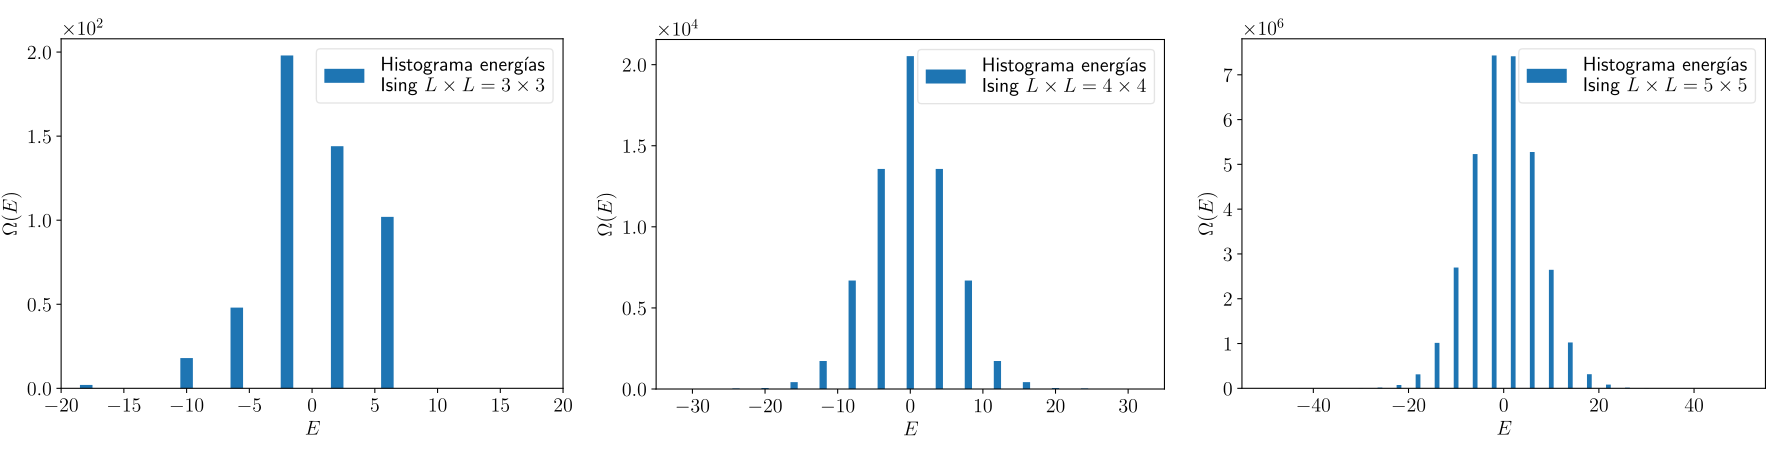
\includegraphics[width=\linewidth]{{{figures/ising-energy-plots-L_3_4_5}}}
			\caption{De izquierda a derecha: histograma de $\Omega(E)$ para $L = 3, \,\,\,4, \,\,\,5$, respectivamente, con condiciones de frontera periódicas. Notamos la asimetría evidente para $L=3$, simetría para $L=4$ y asimetría no evidente en $L=5$. Este fenómeno se debe a las condiciones de frontera periódicas y es un efecto de tamaño finito, pues para $L$ lo suficientemente grande, el histograma es aproximadamente simétrico independientemente de si $L$ es impar o par.}
			\label{fig:energy-omegas-3x3-4x4-5x5}
		\end{figure}

	Para entender un poco mejor la asimetría en los histogramas con $L$ impar, consideremos momentáneamente el caso de condiciones de frontera libres. En la figura \ref{fig:energy-asymmetry-fbc-3x3} (centro) se muestra dicho histograma para $L=3$. Notamos que el histograma ahora contiene la energía $E=0$ y que es simétrico (no aparentemente sino exactamente simétrico). Para entender mejor el efecto de las condiciones de frontera se muestran en la misma figura configuraciones de menor y mayor energía (izquierda y derecha, respectivamente). Al considerar condiciones de frontera periódicas, para el caso de menor energía (izquierda) con condiciones de frontera libres se tiene $E = -12$ y con condiciones de frontera periódicas, se tiene $E = -18$. Para el caso de mayor energía con condiciones de frontera libres se tiene $E=12$, mientras que en el caso de condiciones de frontera periódicas se tiene $E=6$. 
	
	Este efecto se da para el caso impar ya que al tener condiciones de frontera periódicas, en el caso de mayor energía, los vecinos de los sitios de los bordes tienen el mismo valor de espín, lo cual hace que la energía disminuya con respecto al valor absoluto de la energía menor del sistema y así se genera la asimetría, es decir $E_{\mathrm{max}} = |E_{\mathrm{min}}| - \Delta E$. Dicho $\Delta E$ está relacionado con las condiciones de frontera. $\Delta E = 0$ para condiciones de frontera libres, lo cual genera la simetría en ese caso y es fácil ver que $ \Delta E = 2 L $ para condiciones de frontera periódicas. La asimetría se `pierde' con $L\rightarrow\infty$ ya que para condiciones de frontera periódicas $E_\mathrm{min} = - 2 L^2$, luego 
		\begin{align}
			E_{\mathrm{max}} &= 2(L^2 - L) \nonumber	\\
			\implies \frac{E_{\mathrm{max}}}{L} &= 2(L - 1) \nonumber \\
												&\approx 2L = \frac{|E_\mathrm{min}|}{L}.
		\end{align}
	Por otro lado, este efecto no se presenta en el caso $L=\mathrm{par}$, ya que todos los vecinos de los sitios de los bordes son de signos diferentes. 

		\begin{figure}[!ht]
			\centering
			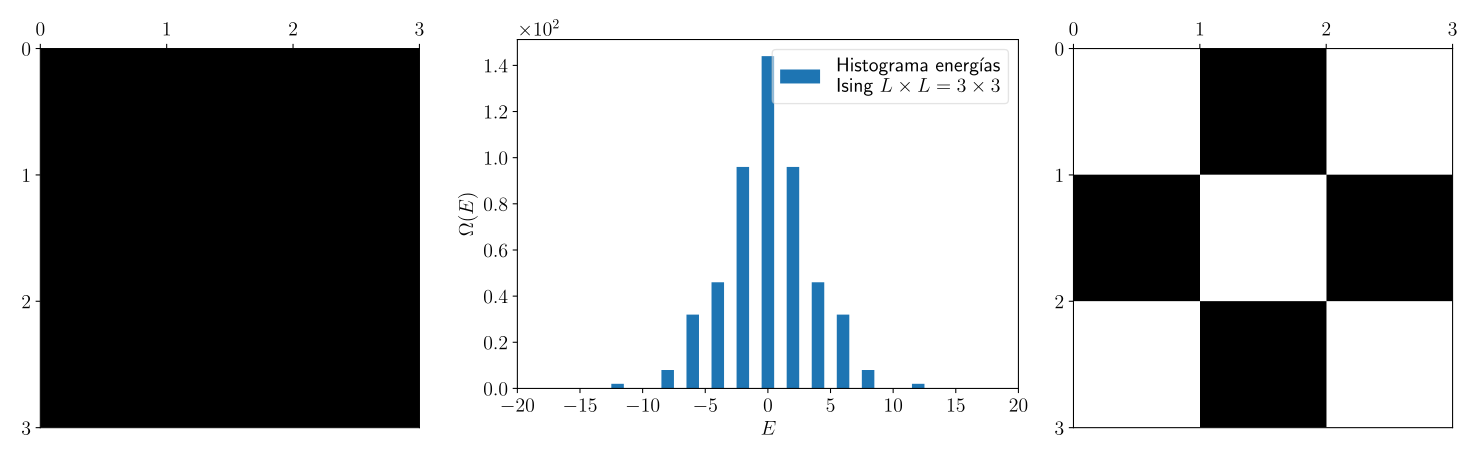
\includegraphics[width=\linewidth]{{{figures/ising-odd_asymmetry-L_3}}}
			\caption{Centro: histograma $\Omega(E)$ para el caso $L=3$ con condiciones de frontera periódicas. Izquierda: un microestado de menor energía (independientemente de las condiciones de frontera). Derecha: un microestado de mayor energía (independientemente de las condiciones de frontera).}
			\label{fig:energy-asymmetry-fbc-3x3}
		\end{figure}

		\begin{figure}[!ht]
			\centering
			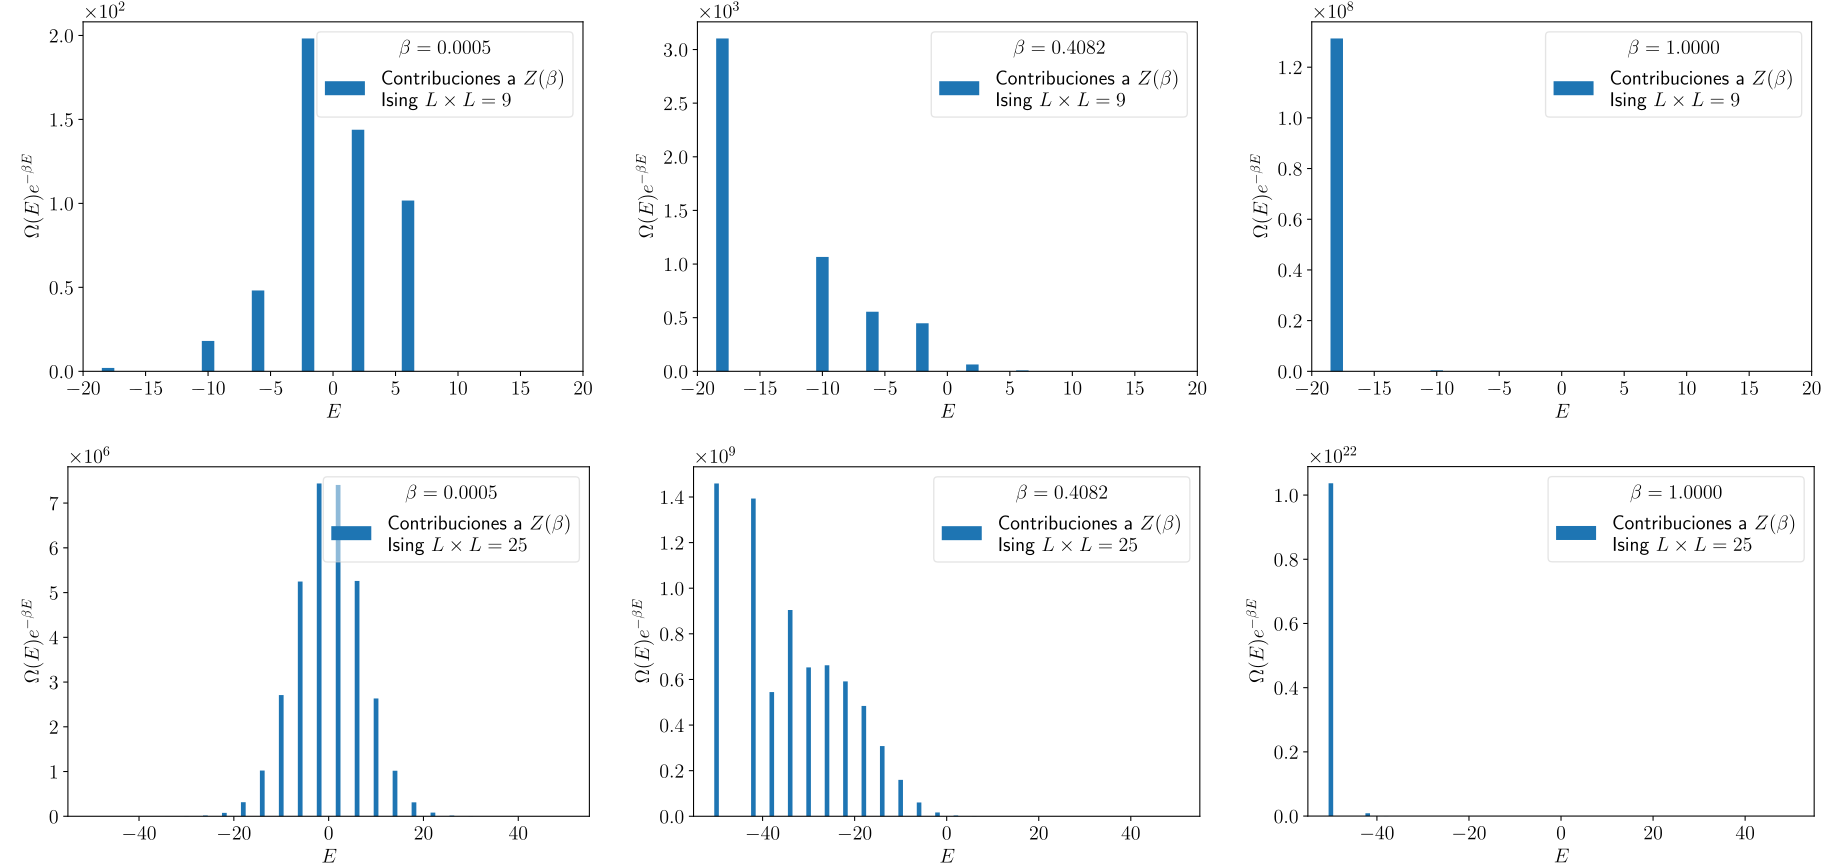
\includegraphics[width=0.9\linewidth]{{{figures/ising-Z_contributions-plots-L_3_5}}}
			\caption{Contribuciones por energías a la función partición $\Omega(E)e^{-\beta E} \propto p_E$. Arriba: $N = 3 \times 3$, abajo: $N = 5 \times 5$. Izquierda: $T=2000$, centro: $T=T_c \approx 2.45$ (temperatura crítica para valores pequeños de $L$), derecha: $T=1$.}
			\label{fig:Z-contributions-L_3_5}
		\end{figure}

	Por otro lado, sabemos que la función partición tiene gran importancia en la física estadística, ya que de ella se deduce la termodinámica del sistema. Notemos que las contribuciones de cada energía a la función partición, \textit{i.e.} $\Omega(E)e^{-\beta E}$ son proporcionales a la probabilidad $p_E$ definida en \ref{eq:energy_prob}. Conocerlas es básicamente conocer la probabilidad de que el sistema se encuentre en una energía $E$ dada.

	En la figura \ref{fig:Z-contributions-L_3_5} mostramos dichas contribuciones por energías a la función partición $\Omega(E)e^{-\beta E} \propto p_E$. Arriba: $N = 3 \times 3$, abajo: $N = 5 \times 5$. Izquierda: $T=2000$, centro: $T=T_c \approx 2.45$ (temperatura crítica para valores pequeños de $L$), derecha: $T=1$. Para temperaturas muy altas, notamos, al comparar con la figura \ref{fig:energy-omegas-3x3-4x4-5x5} que los histogramas son casi idénticos. Esto es esperable ya que $T \gg 0 \implies \beta \ll 1 \implies \Omega(E) e^{-\beta E} \approx \Omega(E)$. Por otro lado, cuando $T \approx T_c$ se tiene que hay mayores contribuciones de energías pequeñas pero aún hay muchas energías que contribuyen al sistema y las contribuciones son mayores cuanto menor es $E$. Éste es es un límite intermedio entre bajas y altas temperaturas, de algún modo $T_c$ se convierte en una temperatura característica del sistema. Finalmente, el límite de bajas temperaturas es el esperado: prácticamente la única contribución es la del estado base.

	\subsection{Equivalencia entre ensambles microcanónico y macrocanónico\label{subsec:teoria-equivalencia-micro}}
	Usualmente encontramos en los textos de física estadística que en el caso del límite termodinámico hay una equivalencia entre los ensambles canónico y microcanónico, que se puede escribir en la forma
		\begin{equation}
			Z(\beta) = \sum_E \Omega(E) e^{-\beta E} \approx \Omega(\langle E \rangle) e^{-\beta \langle E \rangle} = Z(\beta)_{\mathrm{appx}} \label{eq:equiv-micro-macro}
		\end{equation}
	Aunque en esta sección no podemos calcular $Z(\beta)$ para sistemas muy grandes (por capacidad computacional solo se logró hacer hasta $L=5$), se realizó una aproximación a este problema, para ver en cuáles son las condiciones en las cuales la expresión anterior se cumple en casos de baja dimensionalidad ($L$ pequeño). El método usado fue, para cada $\beta$ y $L$ calcular la energía promedio $\langle E \rangle$, posteriormente se interpoló linealmente los histogramas de la figura \ref{fig:energy-omegas-3x3-4x4-5x5} para obtener $\Omega(\langle E \rangle)$ y con esto se calculó $Z_\mathrm{appx}$ definida en (\ref{eq:equiv-micro-macro}).

	En la figura \ref{fig:micro-macro-equivalence}, con líneas punteadas se muestra el resultado del método $\log Z_\mathrm{appx}$ y con líneas continuas el valor real calculado directamente, $\log Z$. En general, encontramos que para temperaturas bajas \textit{i.e.} $\beta$ alto, la equivalencia se da casi de inmediato. Esto se debe básicamente a que la energía mínima es la más dominante en el sistema (por gran diferenca con respecto a las demás) y es muy cercana a la energía promedio. Por tanto, el sistema tiene prácticamente energía constante (casi sin fluctuaciones) \textit{i.e.} el ensamble canónico y el microcanónico son equivalentes. Para poder concluir acerca de la validez de (\ref{eq:equiv-micro-macro}) en el límite termodinámico es necesario hacer este estudio para $L$ grandes, lo cual está por fuera de nuestras capacidades de cómputo. 
		
		\begin{figure}[!ht]
			\centering
			\includegraphics[width=0.6\linewidth]{{{figures/ising-Z_approx-plot-L_2_3_4_5}}}
			\caption{En líneas punteadas se muestra $\log Z_\mathrm{appx}$ calculado con el método descrito en el artículo y en líneas continuas $\log Z$ calculado directamente por enumeración exacta. Esto muestra la equivalencia a bajas temperaturas entre ensambles microcanónico y macrocanónico en el caso de bajo valor $L$, expresada por la ecuación (\ref{eq:equiv-micro-macro}).}
			\label{fig:micro-macro-equivalence}
		\end{figure}

	\subsection{Calor específico\label{subsec:teoria-calor-especifico}}
	
	\begin{figure}[!ht]
		\centering
		\includegraphics[width=0.6\linewidth]{{{figures/ising-specific_heat-plot-L_2_3_4_5}}}
		\caption{Calor específico $c_v$ dado por (\ref{eq:cv-fluctuation}) en función de la temperatura para diferentes valores de $L$. Los picos corresponden con la `temperatura crítica', que para $L$ grande se convierten en puntos discontinuos, demostrando así una transición de fase de segundo orden en el sistema.}
		\label{fig:specific-heat}
	\end{figure}

	\begin{figure}[!ht]
		\centering
		\includegraphics[width=0.6\linewidth]{{{figures/ising-cv-computation_time}}}
		\caption{Tiempo de cómputo para las gráficas de calor específico y ajuste exponencial para predecir tiempo de cómputo para el sistema $N = 8 \times 8$. Suponiendo que se tiene la memoria RAM necesaria, el proceso de obtención de la gráfica $c_v(T)$ para dicho sistema sería aproximadamente 47 mil días o 128 años.}
		\label{fig:cv-comp-time}
	\end{figure}

	Con las probabilidades para las energías del sistema dadas por (\ref{eq:energy_prob}) es fácil calcular el valor medio de $E$ y el valor medio de $E^2$
		\begin{eqnarray}
			\langle E \rangle &=& \sum_E E p_E = \sum_E E \frac{\Omega(E) e^{-\beta E}}{Z} \\
			\langle E^2 \rangle &=& \sum_E E^2 p_E = \sum_E E^2 \frac{\Omega(E) e^{-\beta E}}{Z}.
		\end{eqnarray}
	Con esto en mente es fácil calcular el calor específico, que en el ensamble canónico está dado por
		\begin{equation}
			c_v = \frac{\beta ^ 2}{N} \left(\langle E^2 \rangle - \langle E \rangle^2 \right). \label{eq:cv-fluctuation}
		\end{equation}

	De los cálculos en las secciones anteriores tenemos todos los elementos para calcular este calor específico para $L = 2,\,\,\, 3,\,\,\, 4,\,\,\, 5$. La figura \ref{fig:specific-heat} muestra dichos valores en función de la temperatura, T. Como nos encontramos aún en valores relativamente bajos de $L$, no se presenta una discontinuidad evidente en el calor específico. Sin embargo, conforme se aumenta $L$, notamos que el pico de $c_v$ se va haciendo más puntiagudo. Para valores más altos de $L$, como se verá en la sección \ref{sec:metropolis}, el pico se convierte en el punto de discontinuidad, demostrando así una transición de fase de segundo orden, para la cual, en el límite $L\rightarrow\infty$, la temperatura crítica es $T_c = 2/\log(1 + \sqrt{2})$. En las gráficas se muestran los valores $T_c$ para cada $L$, asociados a los picos de las gráficas.
	
	En la última figura de esta sección, \ref{fig:cv-comp-time}, presentamos un ajuste exponencial para los tiempos de cómputo de las gráficas $c_v(L)$ para cada $L$. El ajuste predice un tiempo de cómputo de 47000 días para el sistema $8 \times 8$. Aquí notamos la inminencia de la complejidad computacional de este problema, que es de tipo exponencial y la incapacidad de tratarlo de forma directa `contando microestados' como lo hemos hestado haciendo hasta ahora. En la siguiente sección presentaremos el algoritmo metrópolis que nos ayudará a aproximarnos a las soluciones de este problema para sistemas más grandes.
		

\section{Modelo de Ising y Algoritmo Metrópolis\label{sec:metropolis}}

En trabajos anteriores ya hemos estudiado el algoritmo Metrópolis, el cual consiste en un muestreo inteligente de distribuciones de probabilidad y que es muy útil para sistemas que presentan un alto número de configuraciones posibles. A continuación explicaremos la implementación de este algoritmo en el caso del modelo de Ising.

	\subsection{El algoritmo Metrópolis para el modelo de Ising 2d\label{subsec:metropolis-algoritmo}}
	
	En esta sección mostramos el retazo de programa más importante que usamos en nuestra implamentación y que corresponde con el algoritmo Metrópolis para el modelo de Ising.

	En la línea 3 importamos el módulo \mintinline{python}{ising2d_metropolis} que escribimos y contiene todas las funciones necesarias para generar las gráficas que se muestran en esta y las siguientes secciones (las gráficas se generaron con el script \mintinline{python}{ising2d_metropolis_run.py} que se puede encontrar en el anexo \ref{appx:montecarlo})

	La línea $11$ calcula los vecinos de cada uno de los sitios que se necesitarán para calcular las energías de cada configuración. El método del cálculo de los vecinos se explica directamente en los comentarios del módulo \mintinline{python}{ising2d_metropolis} y consiste en tener en cuenta las condiciones de frontera periódicas de manera compacta usando operadores división suelo (\textit{floor division}) y módulo.

	Las líneas $14-17$ deciden si se leyó un microestado inicial para comenzar el algoritmo o si se generará uno de forma aleatoria.

	La línea 20 calcula la energía del microestado inicial.

	Las líneas $26-32$ corren el algoritmo Metrópolis para un número de pasos transiente \mintinline{python}{N_transient}, con el fin de que el sistema se termalice. En esta parte NO se guardan los datos de las energías de cada paso, precisamente porque es una etapa de transiente y no muestra las características del estado de equilibrio, en el cual estamos interesados. La probabilidad de aceptación es dada por la razón de los factores de boltzmann del microestado propuesto sobre el microestado anterior, ya que estamos trabajando en el ensamble canónico.

	Las líneas $34-41$ corren el algoritmo Metrópolis para un número de pasos \mintinline{python}{N_steps}, en el cual se espera que el sistema ya esté termalizado, es decir, que se encuentre en un estado de equilibrio del ensamble canónico. En esta parte se guardan las energías de cada configuración por la que pasa el sistema. El resultado final del algoritmo es una lista con las energías por las cuales pasó el sistema durante el número de pasos \mintinline{python}{N_steps}, éstas constituyen un muestreo inteligente de la distribución de probabilidad $p_E$ dada por (\ref{eq:energy_prob}) y por tanto nos permiten calcular las propiedades termodinámicas del sistema.
	
	El resto del módulo \mintinline{python}{ising2d_metropolis} está bien explicado en los comentarios del mismo.

	Hay que anotar enfáticamente que en las implementaciones del algoritmo metrópolis se usó la librería Numba que permite un tipo de compilación de los programas denominado JIT (\textit{Just In Time Compilation}). Sin el uso de esta librería, no hubiese sido posible el cálculo tan preciso de las datos usados para generar las gráficas acá presentadas, ya que los tiempos de cómputo al usar este tipo de compilación permiten ganancias en la optimización de los tiempos de cómputo hasta en 100 veces \cite{10.1145/2833157.2833162}.

		\inputminted[linenos,breaklines]{python}{ising2d-metropolis-z-retazo.py}


	\subsection{Importancia de la termalización del sistema al usar el algoritmo Metrópolis\label{subsec:metropolis-termalizacion}}

	Como se dijo en la sección anterior, se espera que en la primera parte del algoritmo (en los primeros \mintinline{python}{N_transient} pasos) el sistema se termalice. Como estamos en el ensamble canónico, la termalización del sistema está caracterizada por la energía promedio del sistema $\langle E \rangle / N$. Cuando esta cantidad se mantenga aproximadamente constante con el cambio del número de iteraciones, podemos asegurar que el sistema se habrá termalizado.

	\begin{figure}[!ht]
		\centering
		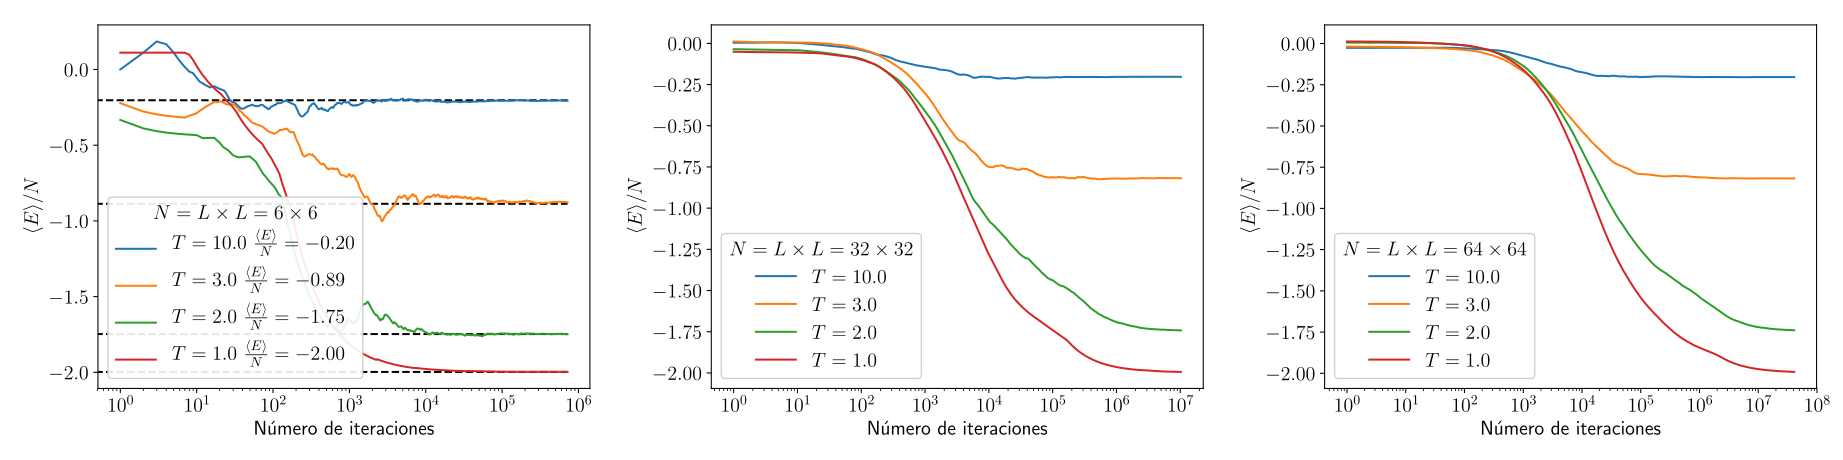
\includegraphics[width=\linewidth]{{{figures/ising-metropolis-thermalization-plot-L_6_32_64-T_10.0_3.0_2.0_1.0}}}
		\caption{Visualización gráfica del paso al equilibrio en el algoritmo Metrópolis para el modelo de Ising en el ensamble canónico, medido por el paso al equilibrio de la energía promedio del sistema. Izquierda: $N=6 \times 6$. Centro: $N=32 \times 32$. Derecha: $N=64 \times 64$.}
		\label{fig:thermalization-energy}
	\end{figure}

	Para entender mejor lo anterior, en la figura \ref{fig:thermalization-energy} se muestra $\langle E \rangle / N$ en función del número de iteraciones \mintinline{python}{N_steps}. Como en este caso estamos interesados en ver direectamente la termalización, se escoge \mintinline{python}{N_transient} igual a cero. En la izquierda se muestra la termalización para el caso $N = 6 \times 6$, en el cual se puede hacer la comparación de $\langle E \rangle / N$ para diferentes teperaturas por enumeración exacta, ya que en el enunciado de la parte 1 se dio el histograma $\Omega(E)$ para este caso y eso basta para calcular $\langle E \rangle / N$. En dicha figura se muestran los valores para cada temperatura y notamos que la termalización se da en escalas diferentes, dependiendo de la temperatura. Así, para temperaturas altas, el sistema se termaliza mucho más rápido que para temperaturas bajas, pero esto es más evidente en sistemas con $L$ más grande. Es interesante notar que los límites están bien definidos. Para temperaturas bajas, el sistema tiende a estados ferromagnéticos que implican  $\langle E \rangle / N \approx -2$, mientras que para temperaturas altas el sistema se termaliza en $\langle E \rangle / N$ cada vez más cercano a cero, como se espera, según los histogramas de $\Omega(E)$ y $e^{-\beta E}\Omega(E)$ mostrados en la sección \ref{subsec:teoria-contribuciones-Z}.
	
	En el centro de la figura \ref{fig:thermalization-energy} encontramos la termalización para $L=32$ y diferentes temperaturas. Notamos que en general la termalización demora más que para el caso anterior ($N = 6 \times 6$). Esto es esperable, ya que el número de configuraciones posibles en este caso ($\Omega = 2^{32 \times 32}$ !!!) es muchísimo mayor que el número de configuraciones en el caso anterior, por lo cual, el sistema debe pasar primero por muchos más estados antes de llegar al equilibrio. Sucede de forma similar con el caso $N=64 \times 64$, el cual necesita muchas más iteraciones para llegar al equilibrio.

	\begin{figure}[!ht]
		\centering
		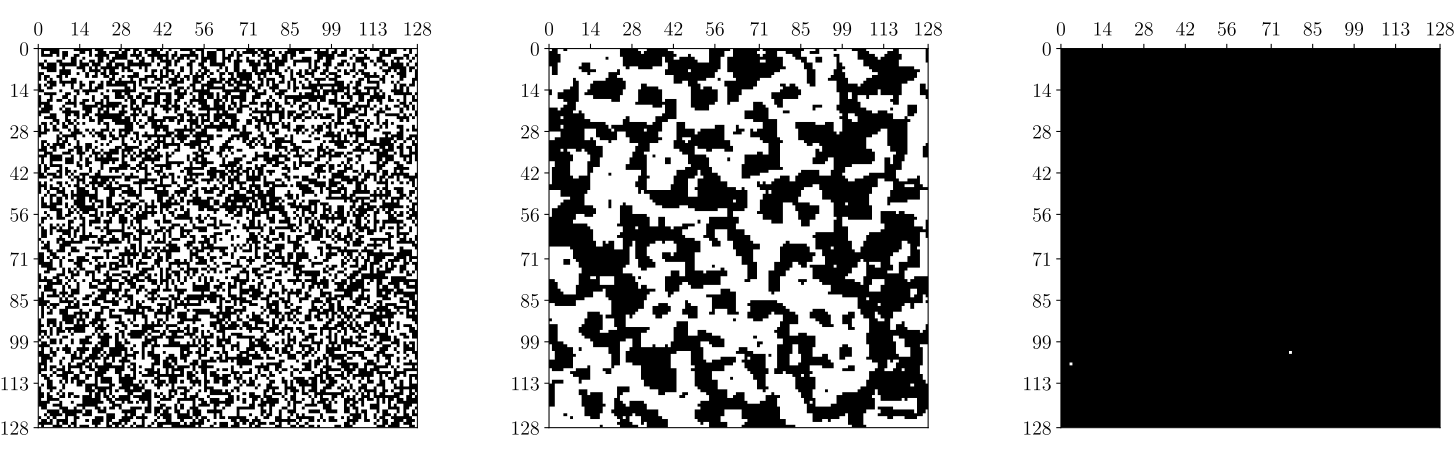
\includegraphics[width=\linewidth]{{{figures/ising-metropolis-config-plot-L_128-thermalization}}}
		\caption{Microestados por los cuales pasa el sistema de $N=128 \times 128$ en el principio del transiente ($\mathrm{N_{steps}}=10^3$, izquierda), en medio del transiente ($\mathrm{N_{steps}}=10^5$, centro) y cuando el sistema ya está termalizado ($\mathrm{N_{steps}}=10^8$, derecha).}
		\label{fig:thermalization-configs}
	\end{figure}
	
	Para ilustrar un poco mejor el tema de la termalización, en la figura \ref{fig:thermalization-configs} mostramos los microestados por los cuales pasa el sistema de $N=128 \times 128$ en el principio del transiente ($\mathrm{N_{steps}}=10^3$), en medio del transiente ($\mathrm{N_{steps}}=10^5$) y cuando el sistema ya está termalizado ($\mathrm{N_{steps}}=10^8$), todo para temperatura baja $T=1$ y, como queremos ver explícitamente la termalización, se usó $\mathrm{N_{transient}}=0$. Vemos que el sistema pasa de una configuración prácticamente aleatoria ($\langle E \rangle / N \approx 0$), luego una configuración con pequeños parches con dominio ferromagnético ($\langle E \rangle / N \approx -1$) y finalmente a una configuración casi completamente ferromagnética donde ($\langle E \rangle / N \approx -2$), estos valores se deducen aproximadamente a partir de la figura \ref{fig:thermalization-energy} (derecha) que muestra la termalización para el caso más cercano al $N = 128 \times 128$ que se pudo obtener.

	\subsection{Microestados finales y temperatura crítica\label{subsec:metropolis-microestados-temp-critica}}

	Una  vez el sistema está termalizado, podemos obtener microestados típicos del modelo de Ising en el ensamble canónico a una temperatura fija. En la figura \ref{fig:final-thermalized-microstates-different-temperatures} encontramos los microestados mencionados del sistema $L=64$ para temperaturas $T = 1,\,\, 2.5\text{ y } 10$ –izquierda, centro y derecha, respectivamente. 
	
	\begin{figure}[!ht]
		\centering
		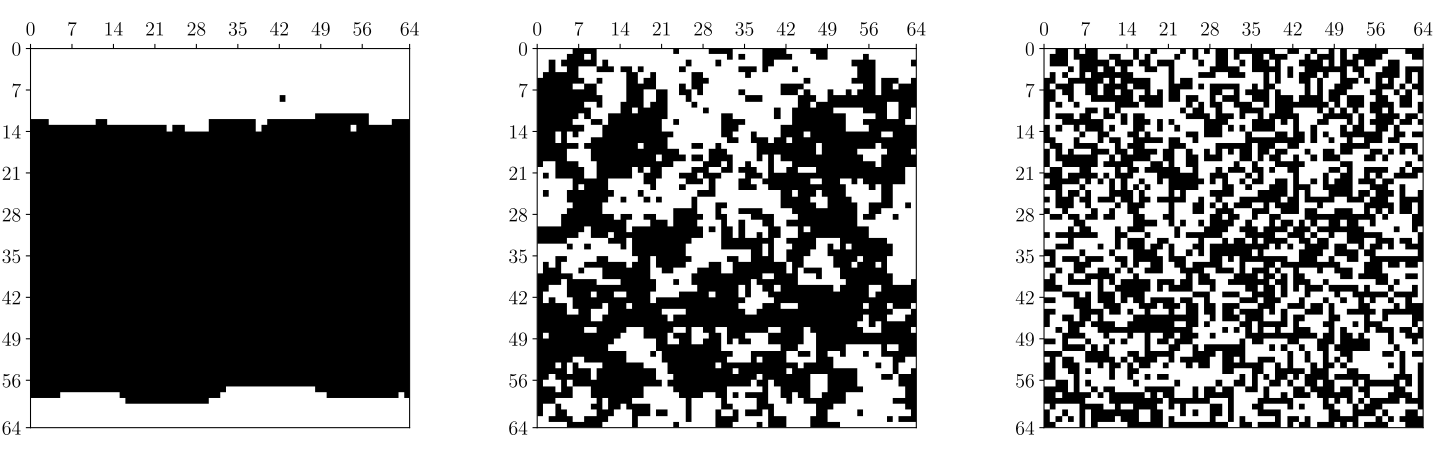
\includegraphics[width=\linewidth]{{{figures/ising-metropolis-config-plot-L_64-temp_1.000_2.500_10.000-typical}}}
		\caption{Microestados típicos del sistema $L=64$ para temperaturas $T = 1,\,\, 2.5\text{ y } 10$ –izquierda, centro y derecha, respectivamente.}
		\label{fig:final-thermalized-microstates-different-temperatures}
	\end{figure}

	Para $T=1$ encontramos un sistema con dos grandes dominios ferromagnéticos, esta configuración es estable a bajas temperaturas para sistemas con $L$ grande, ya que el aumento en la energía debido a los bordes entre los dos diferentes dominios ferromagnéticos aumentan poco la energía del sistema \textit{i.e} $\delta E>0$ de los bordes es mucho menor a la energía de un sistema con un solo dominio ferromagnético $E_\mathrm{min}=-2L^2<0$. Cuanto más baja sea la temperatura, este tipo de microestados con dos grandes dominios ferromagnéticos serán menos probables y en cambio serán mucho más probables microestados con un solo dominio ferromagnético (todos los espines $1$ o todos $-1$).

	El caso $T=2.5$ es más cercano a la temperatura crítica del sistema con $L$ infinito. Aquí observamos que hay pequeños pero muchos más dominios ferromagnéticos (pequeños parches blancos o negros), que corresponden con un sistema típico de temperatura que no es muy alta ni muy baja.

	Finalmente, el caso de alta temperatura, $T=10$ es casi completamente aleatorio, aunque aún se notan algunos dominios ferromagnéticos son casi imperceptibles. Este es un microestado típico de alta temperatura, donde todos los microestados son casi igualmente probables y en el que predominan energías promedio $\langle E \rangle / N$ cercanas a cero, como se puede ver en la figura \ref{fig:thermalization-energy} (derecha). \newline
	

	Un caso interesante de estudio son las configuraciones típicas de un sistema relativamente grande a temperatura cercana a la temperatura crítica. Para entender qué sucede en este caso, en la figura \ref{fig:final-critical-temp-128x128} se muestran tres configuraciones típicas para el sistema $L=128$ a tempreatura $T_c \approx 2.27$. Encontramos que a esta temperatura hay grandes dominios ferromagnéticos que ya están prácticamente formados pero contienen ``ruido'' en su interior, es decir, grandes regiones blancas o negras que en su interior contienen esporádicamente el color (espín) contrario. Esta es la manifestación del cambio de fase de segundo orden, de la cual ya hablamos en la sección \ref{subsec:teoria-calor-especifico}. Para temperaturas menores a la temperatura crítica esperamos obtener menos ruido en esos dominios ferromagnéticos bien formados, paulatinamente hasta llegar a un estado totalmente ferromagnético en el límite $T \rightarrow 0$. Para temperaturas más altas, esperamos tener estados un poco más aleatorios con dominios ferromagnéticos cada vez menos evidentes. 

	\begin{figure}[!ht]
		\centering
		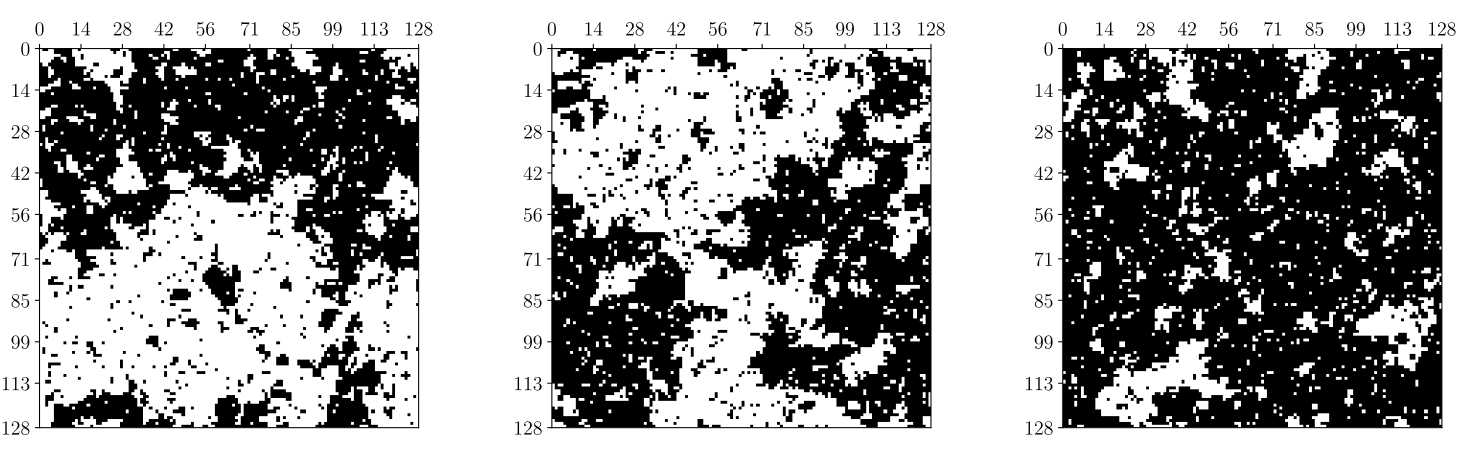
\includegraphics[width=\linewidth]{{{figures/ising-metropolis-config-plot-L_128-temp_2.270-critical-temp}}}
		\caption{Tres configuraciones típicas para el sistema $L=128$ a tempreatura $T_c \approx 2.27$.}
		\label{fig:final-critical-temp-128x128}
	\end{figure}

	\subsection{Calor específico\label{subsec:metropolis-cv}}
	Para finalizar nuestros análisis, presentamos en la figura \ref{fig:metropolis-cv} el calor específico calculado para varios valores de $L$, hasta $L=64$. En primer lugar hay que mencionar que obtener esta gráfica no sería posible de manera sencilla por enumeración exacta ya que el número de microestados $\Omega = 2^{64 \times 64}$ es un número casi inconmesurable que sobrepasa cualquier capacidad computacional. En cambio, mediante un muestreo inteligente con el algoritmo metrópolis es posible obtenerla. En los casos $L = 2,\text{ }3,\text{ }4\text{ y }5$ se muestra para comparación y en línea negra punteada los resultados obtenidos por enumeración exacta. Notamos que el algoritmo metrópolis logra capturar estas curvas con gran precisión.

	Para valores más grandes de $L$ no es posible obtener la curva `teórica' ya que no se tiene acceso a la ennumeración exacta de los microestados. Sin embargo, notamos que las curvas para estos valores son continuas y presentan pocas fluctuaciones, lo cual da un buen presagio para la exactitud del método. 

	Encontramos también evidente que el pico de las gráficas se hace cada vez más puntiagudo, conforme aumenta $L$, lo cual evidencia una transición de fase de segundo orden, según se comentó ya en la sección \ref{subsec:teoria-calor-especifico}.

	\begin{figure}[!ht]
		\centering
		\includegraphics[width=0.6\linewidth]{{{figures/ising-metropolis-specific_heat-plot-L_2_3_4_5_8_16_32_64-N_steps_factor_80000}}}
		\caption{Calor específico en función de la temperatura para varios tamaños $L$ del sistema calculados con el algoritmo metrópolis. Se nota que cuanto mayor es $L$, la discontinuidad en la curva $c_v(T)$ comienza a formarse, característica propia de una transición de fase de segundo orden. Los parámetros usados fueron $\mathrm{N_{steps}}= 80000 L \times L$, $\mathrm{N_{transient}}= 0.7 \mathrm{N_{steps}}$ y se graficaron 100 datos de $c_v$ para valores entre $T=1$ y $T=5$. El tiempo de cómputo fue de $12000 \mathrm{s}$.}
		\label{fig:metropolis-cv}
	\end{figure}



\section{Conclusión\label{sec:conclusion}}

El modelo de Ising es un sistema con una gran riqueza conceptual, debido a la sencillez de su planteamiento y a la gran cantidad de información que podemos obtener de él. Esto lo pudimos observar alrededor de todo el artículo. 

La sencillez de su planteamiento no se traduce en sencillez de cómputo, pues como se vio en la primera sección, éste es un sistema en el cual el número de microestados crece muy rápidamente conforme $L$ crece. Sin embargo, para valores pequeños de L fue posible evidenciar características como la asimetría en los histogramas de $\Omega(E)$ para $L$ impar, que lo asociamos a un efecto de tamaño finito debido a las condiciones de frontera periódicas usadas. Pudimos también evidenciar en esta parte que las contribuciones a la función partición son mayores para estados menos energéticos conforme disminuimos la temperatura del sistema, tal y como se espera. Además, encontramos que para temperaturas bajas, a pesar de que $L$ fuese bajo, hay una equivalencia entre los ensambles micro y macrocanónico. En lo que a esto concierne se podría investigar a futuro, con el método Metrópolis si para sistemas con $L$ grande esta equivalencia la podemos evidenciar para cualquier temperatura. Finalmente, para estos sistemas de $L$ pequeño pudimos calcular por enumeración exacta y usando el teorema de fluctuación-disipación las curvas $c_v(T)$ en las que se comienza a dar indicio de la transición de fase de segundo orden, que es mucho más evidente para sistemas con $L$ grande, tal y como se mostró en la sección del algoritmo metrópolis. Evidenciamos también en esta parte que el tiempo computacional para sistemas levemente mayores $L=8$ el tiempo computacional desborda las capacidades de un computador `sencillo'.

Dadas las limitaciones del método de enumeración exacta, nos vimos en la necesidad de acudir a una técnica de muestreo inteligente para poder obtener información de sistemas más grandes (hasta $N=128 \times 128$): el algoritmo Metrópolis nos permitió reproducir gran cantidad de la información obtenida para sistemas pequeños pero para sistemas mucho más grandes. Encontramos que uno de los aspectos más delicados es lograr termalizar el sistema, de manera que los datos obtenidos mediante el algoritmo sean fidedignos. Pudios evidenciar en esta parte configuraciones típicas de microestados a diferentes temperaturas y para diferentes tamaños, encontrando que para temperaturas bajas los sistemas tienden a dominios casi completamente ferromagnéticos, en la temperatura crítica existen pocos y grandes dominios ferromagnéticos con `ruido' que son característicos de la transición de fase y en temperaturas altas, los microestados tienden a ser muy aleatorios. Finalmente pudimos evidenciar mucho mejor la transición de fase de segundo orden como una (casi) discontinuidad en la curva $c_v$ para sistemas con $L$ grande (en nuestro caso logramos llegar hasta $L=64$ y fue suficiente para notar el inicio de la formación de unadiscontinuidad, recordemos que la discontinuidad como tal se nota para $L\rightarrow\infty$).

Es de recalcar que para la parte del algoritmo Metrópolis, el cálculo computacional necesario para obtener las gráficas no hubiese sido posible sin el uso de la librería Numba, como se mencionó en la sección \ref{subsec:metropolis-algoritmo}.

\section*{Agradecimientos}
Agradezco a mis compañeros de clase con los que tuve discusiones que ayudaron en la implementación del algoritmo y en las conclusiones presentadas.

\nocite{*}

\bibliography{5-Semestre_X_2020_I-Fisica_Estadistica_Avanzada-Tarea_3}% Produces the bibliography via BibTeX.



\newpage


\appendix


\section{Código 1: enumeración exacta de microestados\label{appx:microestados}}

A continuación se muestra el código usado para generar las gráficas de la sección \ref{sec:teoria-microestados}. Éste código usa el módulo \mintinline{python}{ising2d_microstates} en el que están todas las funciones que realizan los algoritmos. Éste último código está disponible en \href{https://github.com/jearistiz/Statistical-Physics-Projects/blob/master/3/ising2d_microstates.py}{este link}.

\inputminted[linenos,breaklines]{python}{code_1.py}

\section{Código 2: algoritmo Montecarlo\label{appx:montecarlo}}

A continuación se muestra el código usado para generar las gráficas de la sección \ref{sec:metropolis}. Éste código usa el módulo \mintinline{python}{ising2d_metropolis} en el que están todas las funciones que realizan los algoritmos. Éste último código está disponible en \href{https://github.com/jearistiz/Statistical-Physics-Projects/blob/master/3/ising2d_metropolis.py}{este link}.

\inputminted[linenos,breaklines]{python}{code_2.py}




\end{document}
%
% ****** End of file apssamp.tex ******
